\section{Kiến trúc tổng quan}
\label{sec:architecture-overview}

\subsection{Mô hình kiến trúc hệ thống}
\label{subsec:system-architecture-model}

ProLearning Platform được đề xuất theo mô hình ứng dụng web/mobile có máy chủ ứng dụng tập trung. Thành phần trung tâm là Spring Boot API, chịu trách nhiệm tiếp nhận yêu cầu, xác thực người dùng, kiểm soát quyền truy cập, điều phối nghiệp vụ và kết nối với các dịch vụ hạ tầng. Cách tổ chức này phù hợp với hệ thống học tập có nhiều miền nghiệp vụ liên quan chặt chẽ, trong đó dữ liệu người dùng, học liệu, tiến độ học tập, thông báo và thanh toán cần được quản lý nhất quán. Nền tảng Spring Boot cung cấp mô hình xây dựng ứng dụng máy chủ theo hướng cấu hình rõ ràng, dễ tích hợp với Spring Security, Spring Data JPA và các thành phần xử lý nền~\cite{springbootdocs,springsecurityjwt,springdatajpa}.

Kiến trúc tổng quan của hệ thống gồm các nhóm thành phần chính sau:

\begin{itemize}
    \item \textbf{Client layer:} Bao gồm Web Client và Mobile Client. Web Client phục vụ các thao tác quản lý học liệu, học flashcard, làm bài kiểm tra, theo dõi roadmap và thanh toán. Mobile Client hỗ trợ các phiên học ngắn, truy cập nhanh học liệu và nhận các push notification. Hai client dùng chung REST API và chỉ sử dụng WebSocket/STOMP đối với các chức năng cần tương tác thời gian thực~\cite{springwebsocketstomp}.

    \item \textbf{Application layer:} Spring Boot API là lớp xử lý nghiệp vụ chính. Lớp này bao gồm controller, service, repository, mapper, scheduler, security filter và các adapter tích hợp. Mọi thao tác ghi dữ liệu lõi đều đi qua application layer để đảm bảo kiểm tra quyền, chuẩn hóa dữ liệu và xử lý lỗi thống nhất.

    \item \textbf{Domain contexts:} Backend được chia thành các bounded context như định danh và bảo mật, learning workspace, collaboration, AI learning, review/progress, todo/calendar, pomodoro, notification, payment/subscription, onboarding/appeal và admin/moderation. Cách chia này làm rõ trách nhiệm của từng nhóm chức năng và giảm phụ thuộc chéo giữa các module.

    \item \textbf{AI Service:} AI Service là thành phần do nhóm phát triển để sinh flashcard, sinh đề kiểm tra, giải thích ghi chú, phân tích kiến thức và tạo roadmap học tập. Backend không để client gọi trực tiếp AI Service; thay vào đó backend đóng vai trò điều phối, kiểm tra quyền, parse kết quả và lưu kết quả AI vào tài nguyên học tập tương ứng.

    \item \textbf{Data and infrastructure layer:} PostgreSQL được sử dụng làm cơ sở dữ liệu quan hệ chính, Redis lưu cache và trạng thái ngắn hạn, RabbitMQ hỗ trợ gửi email bất đồng bộ. Ngoài ra, hệ thống tích hợp Cloudinary cho asset, Firebase Cloud Messaging cho push notification, Google OAuth/Calendar cho đăng nhập và đồng bộ lịch, PayOS cho thanh toán~\cite{postgresqlabout,redisoverview,rabbitmqtutorials,cloudinaryjava,firebasefcm,googlecalendarjava,payoswebhook}.
\end{itemize}

Từ góc nhìn triển khai, kiến trúc trên có ba đặc điểm chính:

\begin{enumerate}
    \item \textbf{Tập trung kiểm soát nghiệp vụ tại backend:} Client chỉ đóng vai trò giao diện và không ghi trực tiếp vào cơ sở dữ liệu hoặc dịch vụ ngoài.
    \item \textbf{Tách biệt các tích hợp bên ngoài:} AI Service, FCM, Google Calendar, Cloudinary và PayOS đều được bọc bởi service/adapter riêng để giảm phụ thuộc trực tiếp vào API của bên thứ ba.
    \item \textbf{Phân tách dữ liệu theo đặc tính sử dụng:} Dữ liệu bền vững được lưu ở PostgreSQL; dữ liệu ngắn hạn như token state, cache hoặc session status được lưu ở Redis hoặc bộ nhớ ứng dụng; tác vụ không cần đồng bộ tức thời được chuyển sang scheduler hoặc message queue.
\end{enumerate}

Sơ đồ dưới đây thể hiện thiết kế tổng thể của hệ thống:

\begin{figure}[htbp]
    \centering
    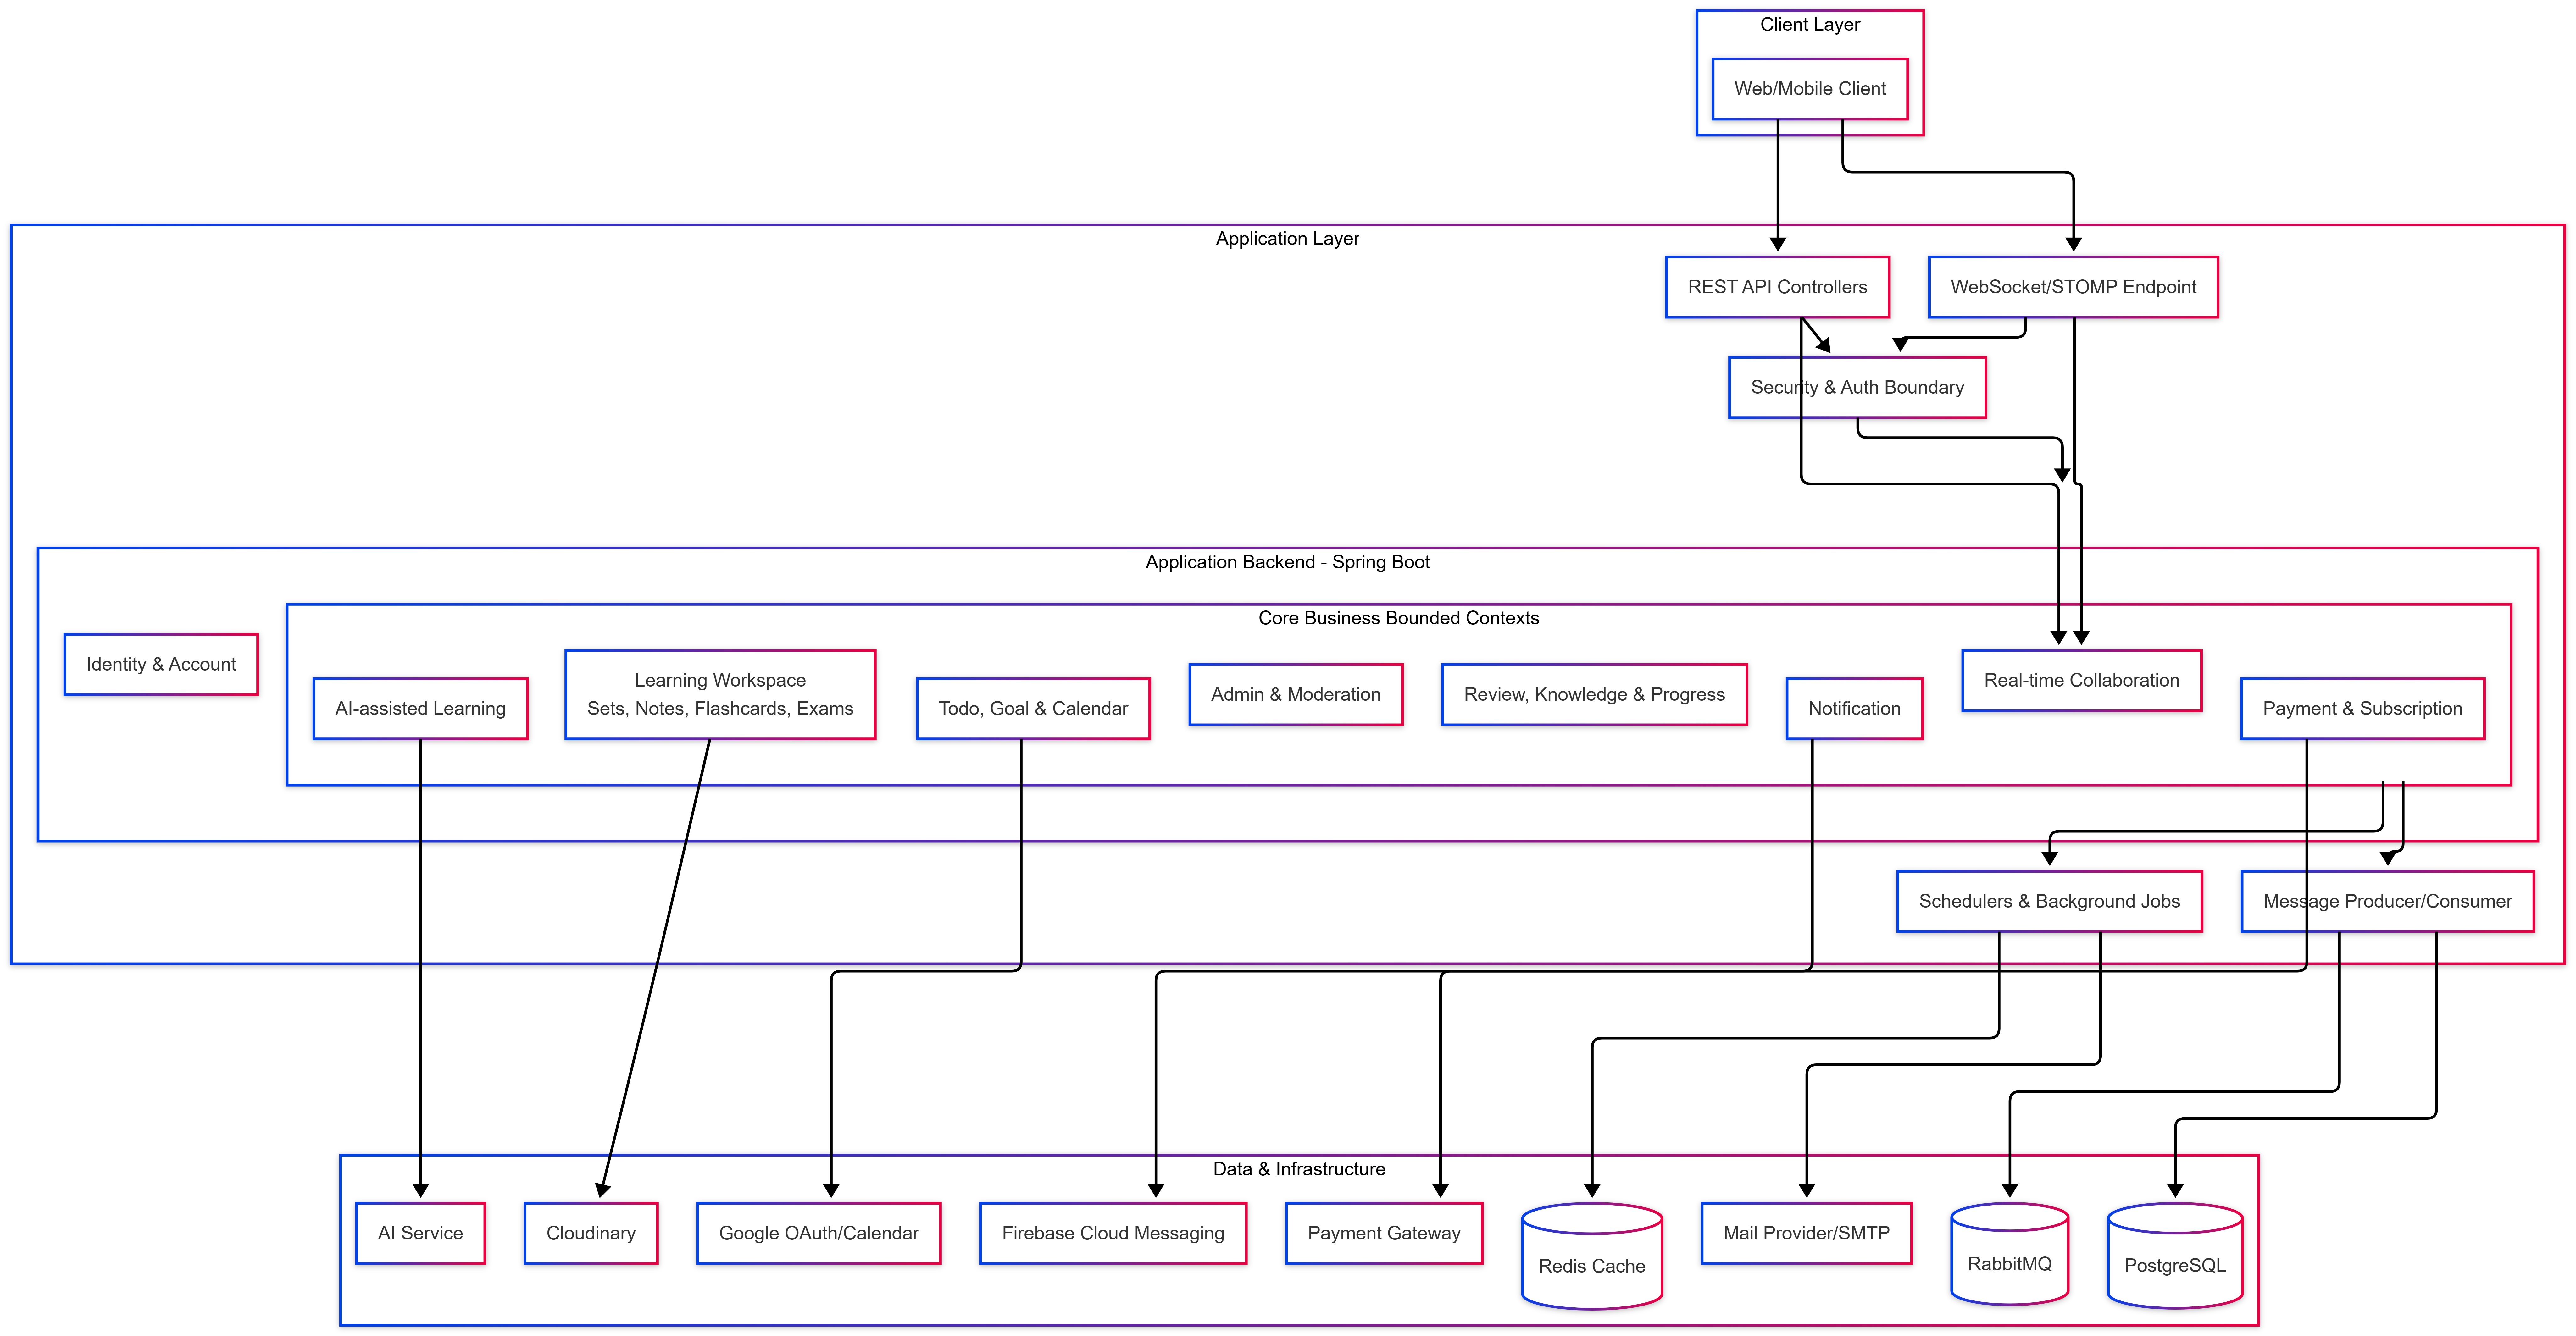
\includegraphics[width=1\textwidth,height=0.95\textheight,keepaspectratio]{images/chapter3/ProLearning_Arch-Overview.drawio.png}
    \caption{Kiến trúc tổng quan của hệ thống ProLearning Platform}
    \label{fig:prolearning-architecture-overview}
\end{figure}